\documentclass[aspectratio=169]{beamer}
\usetheme{metropolis}
\AtBeginSection{}
\usepackage[utf8]{inputenc}
\usepackage[spanish]{babel}
\usepackage{amsmath, amssymb}
\usepackage{graphicx}
\usepackage{tikz}
\usetikzlibrary{shapes.geometric, arrows.meta, positioning, backgrounds}

\setbeamerfont{frametitle}{size=\large}

\title{Fusión de Atención Cruzada para Segmentación del Segmento Anterior}
\subtitle{Usando Representaciones de Imagen Complementarias}
\author[Alfaro · Avilés · Duque]{Caleb Alfaro \and Desireé Avilés \and Danilo Duque}
\institute{Instituto Tecnológico de Costa Rica \\ Redes Neuronales — Grupo PARMA}
\date{Semana 17, 2026}

% ─────────────────────────────────────────────────────────────────────────────
\begin{document}

% ── Secciones (deben ir antes del TOC) ───────────────────────────────────────
\section{Motivación}
\section{Trabajo Relacionado}
\section{Método Propuesto}
\section{Experimentos y Resultados}
\section{Conclusión}

% ── Slide 1: Título ───────────────────────────────────────────────────────────
\begin{frame}
\titlepage
\end{frame}

% ── Slide 2: Agenda ───────────────────────────────────────────────────────────
\begin{frame}{Agenda}
\tableofcontents
\end{frame}

% ══════════════════════════════════════════════════════════════════════════════
%  CALEB — Slides 3–9  (~7 min)
% ══════════════════════════════════════════════════════════════════════════════

% ── Slide 3: El problema clínico ─────────────────────────────────────────────
\begin{frame}{El Problema: Cataratas}
\begin{itemize}
    \item Las cataratas afectan a más de \textbf{100 millones de personas} en el mundo
    \item Es la \textbf{principal causa de ceguera prevenible}
    \item El diagnóstico requiere identificar estructuras del segmento anterior:
    \begin{itemize}
        \item Córnea, pupila, cristalino
    \end{itemize}
\end{itemize}
\vspace{0.5em}
\begin{block}{Necesidad clínica}
Segmentar automáticamente estas estructuras para graduación, planificación quirúrgica y guía intraoperatoria.
\end{block}
\end{frame}

% ── Slide 4: Por qué RGB no es suficiente ────────────────────────────────────
\begin{frame}{¿Por qué RGB solo no es suficiente?}
\begin{columns}
\column{0.55\textwidth}
\begin{itemize}
    \item La opacificación del cristalino genera \textbf{bajo contraste de color}
    \item Las lámparas de hendidura producen \textbf{artefactos de iluminación}
    \item Los modelos unimodales fallan precisamente cuando el paciente está más grave
\end{itemize}
\vspace{0.5em}
\begin{alertblock}{Problema clave}
El color solo no alcanza para delinear los bordes del cristalino opacificado.
\end{alertblock}
\column{0.42\textwidth}
\centering
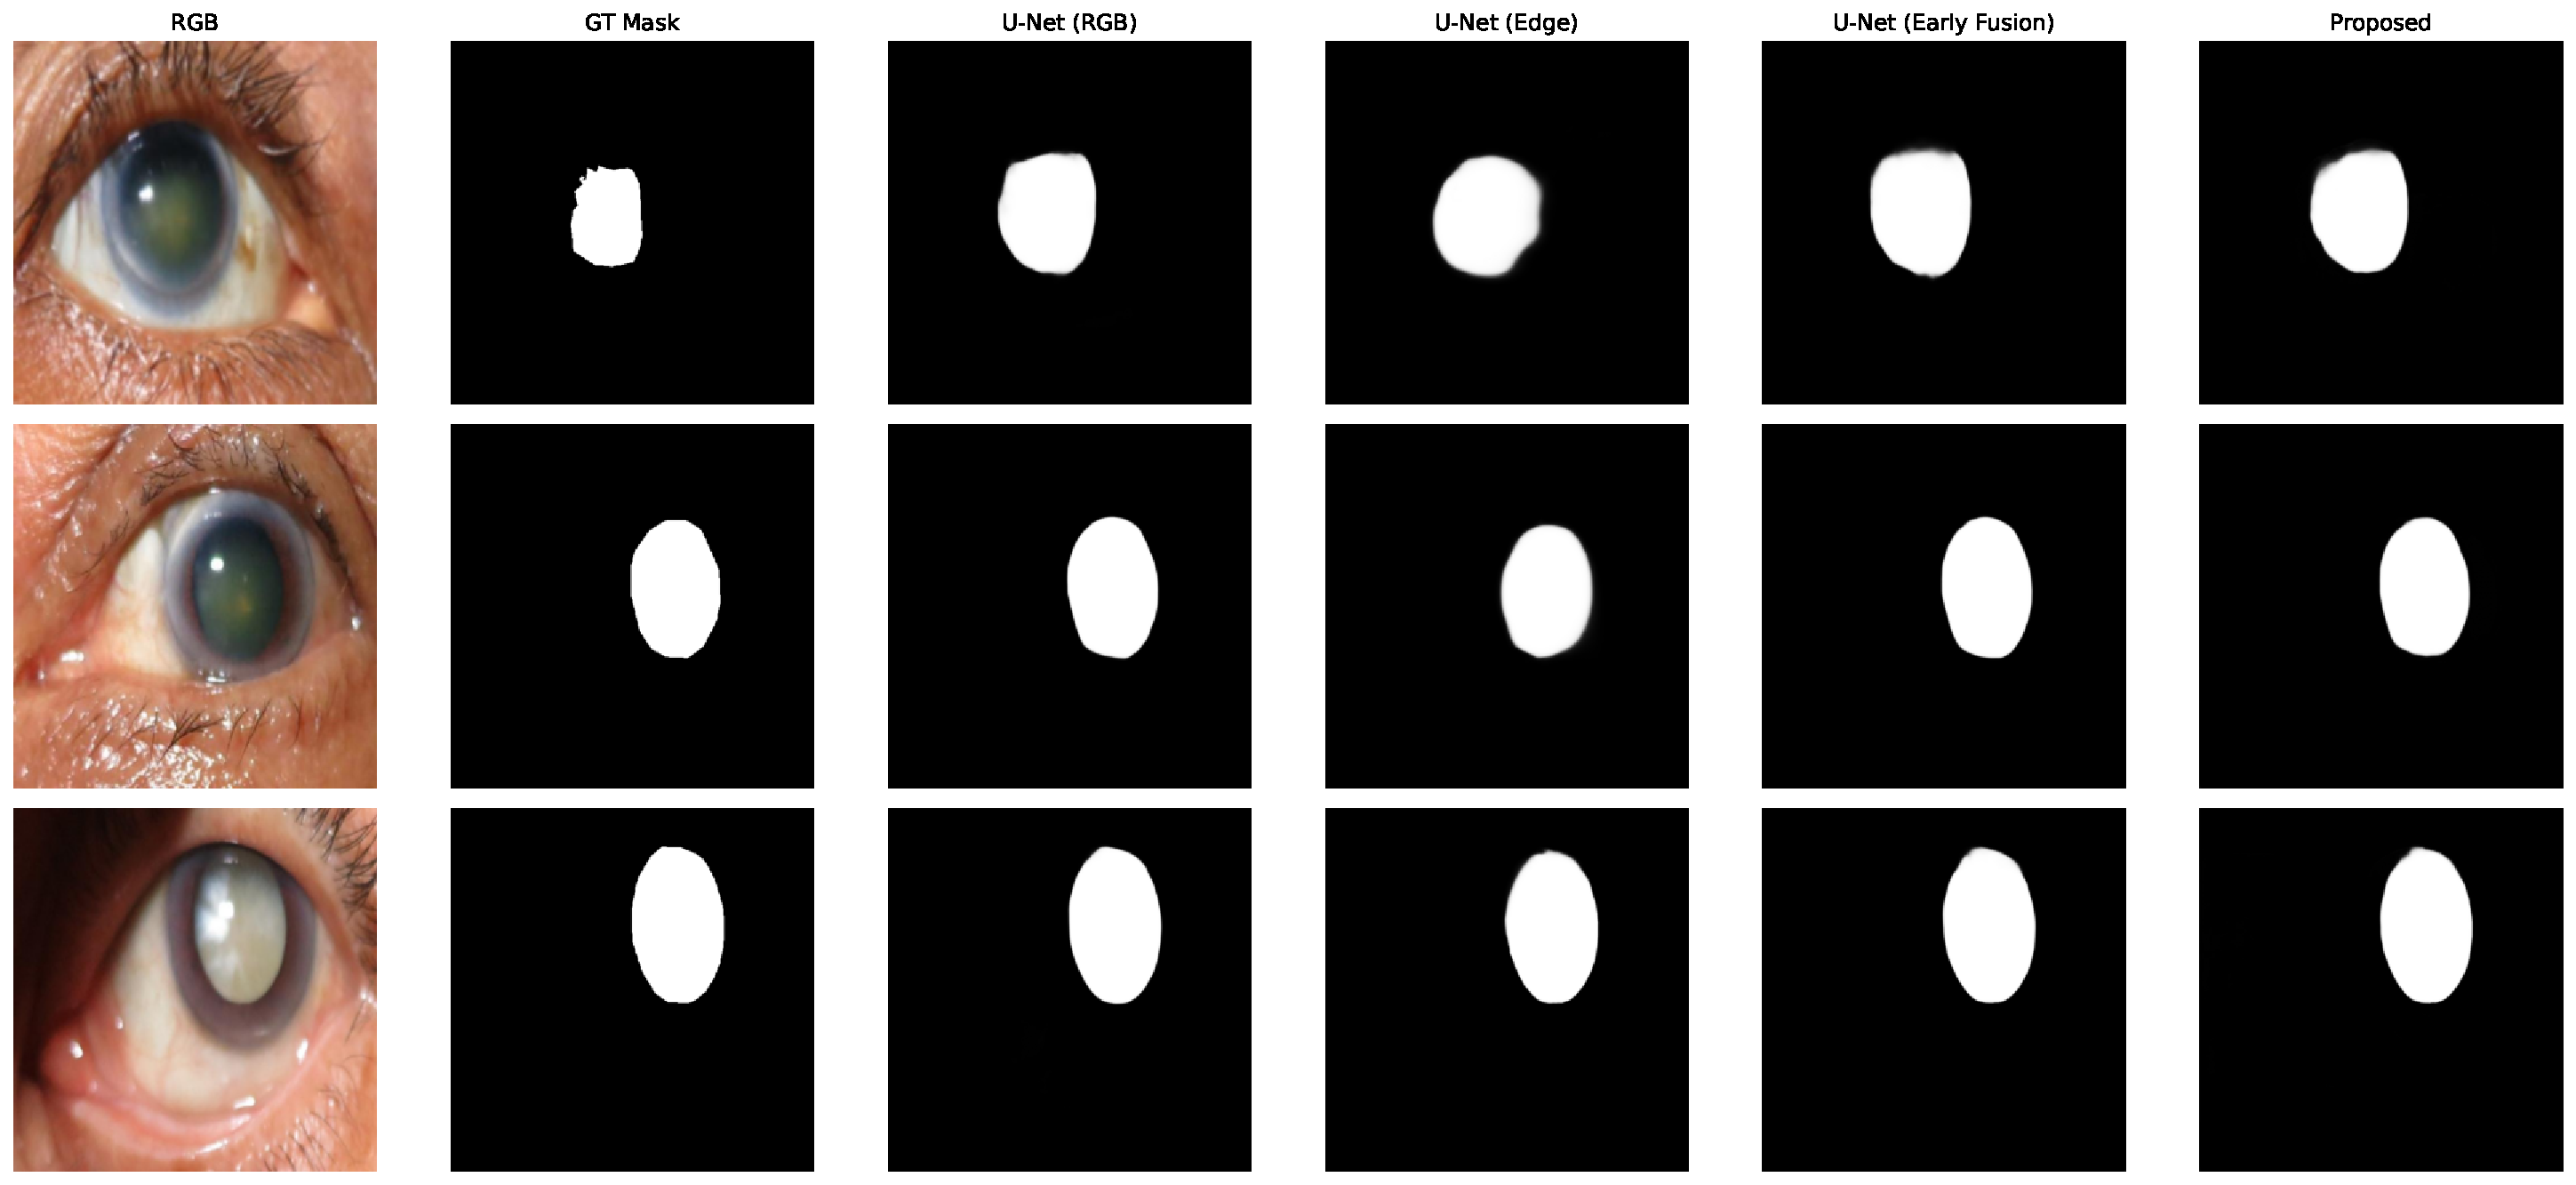
\includegraphics[width=\textwidth]{../paper/figures/qualitative_predictions.pdf}
\end{columns}
\end{frame}

% ── Slide 5: ¿Qué es segmentación multimodal? ────────────────────────────────
\begin{frame}{¿Qué es Segmentación Multimodal?}
\begin{block}{Idea central}
Usar \textbf{múltiples representaciones} de la misma escena y \textbf{fusionarlas} para que el modelo vea más de lo que cualquier vista individual puede capturar.
\end{block}
\vspace{0.6em}
\begin{columns}
\column{0.48\textwidth}
\textbf{Multimodal clásico} (sensores distintos):
\begin{itemize}
    \item MRI T1 + T2 + FLAIR para tumores cerebrales
    \item RGB + profundidad para escenas 3D
\end{itemize}
\column{0.48\textwidth}
\textbf{Nuestro enfoque} (misma imagen, dos vistas):
\begin{itemize}
    \item Imagen RGB $\rightarrow$ features fotométricas
    \item Mapa de bordes Canny $\rightarrow$ features geométricas
    \item Espacios de features heterogéneos $\Rightarrow$ fusión multimodal
\end{itemize}
\end{columns}
\end{frame}

% ── Slide 6: Trabajo Relacionado — Backbone ──────────────────────────────────
\begin{frame}{Trabajo Relacionado: Segmentación Médica}
\begin{itemize}
    \item \textbf{U-Net} \textit{[Ronneberger 2015]} — arquitectura encoder-decoder con skip connections
    \begin{itemize}
        \item Backbone de nuestro modelo
        \item Preserva detalle espacial fino
    \end{itemize}
    \vspace{0.4em}
    \item \textbf{CaDIS} \textit{[Grammatikopoulou 2021]} — benchmark de escenas quirúrgicas de cataratas
    \begin{itemize}
        \item Motivación del dominio
    \end{itemize}
    \vspace{0.4em}
    \item \textbf{MedSAM / SAM-Adapter} \textit{[Ma 2024, Chen 2023]} — modelos fundacionales
    \begin{itemize}
        \item Requieren 20+ GPUs A100 y grandes volúmenes de datos
        \item \textbf{No son viables} para datasets pequeños como el nuestro
    \end{itemize}
\end{itemize}
\end{frame}

% ── Slide 7: Trabajo Relacionado — Fusión ────────────────────────────────────
\begin{frame}{Trabajo Relacionado: Fusión Multimodal}
\begin{itemize}
    \item \textbf{Vaswani 2017} — ``Attention is All You Need''
    \begin{itemize}
        \item Define el mecanismo Q/K/V que adoptamos
    \end{itemize}
    \vspace{0.3em}
    \item \textbf{mmFormer} \textit{[Zhang 2022]} — transformer multimodal médico
    \begin{itemize}
        \item Cross-attention entre modalidades de MRI
        \item \textbf{Inspiración directa de nuestro módulo de fusión}
    \end{itemize}
    \vspace{0.3em}
    \item \textbf{DECTNet} \textit{[Li 2024]} — encoder dual CNN + Transformer
    \begin{itemize}
        \item Precedente estructural: encoders paralelos con sesgos inductivos distintos
    \end{itemize}
\end{itemize}
\end{frame}

% ── Slide 8: Brecha que llenamos ─────────────────────────────────────────────
\begin{frame}{¿Dónde Encaja Nuestro Trabajo?}
\centering
\begin{tikzpicture}[font=\small, node distance=1.2cm]
    \node[draw, rounded corners, fill=blue!10, text width=3.2cm, align=center] (unet)
        {Específico para tarea\\(U-Net)\\Fuerte, pero unimodal};
    \node[draw, rounded corners, fill=orange!15, text width=3.2cm, align=center, right=1.5cm of unet] (fusion)
        {Fusión multimodal\\(mmFormer, DECTNet)\\Solo multi-sensor};
    \node[draw, rounded corners, fill=red!10, text width=3.2cm, align=center, right=1.5cm of fusion] (fm)
        {Modelos fundacionales\\(MedSAM, SAM)\\Inaccesibles en escala};
    \node[draw, rounded corners, fill=green!20, text width=3.8cm, align=center, below=1.2cm of fusion] (ours)
        {\textbf{Nuestro modelo}\\Encoder dual + cross-attention\\Liviano, sin preentrenamiento\\Fusión multimodal intra-imagen};
    \draw[-{Stealth}, thick] (unet.south) -- (ours.west);
    \draw[-{Stealth}, thick] (fusion.south) -- (ours.north);
\end{tikzpicture}
\end{frame}

% ══════════════════════════════════════════════════════════════════════════════
%  DESIREÉ — Slides 9–16  (~7 min)
% ══════════════════════════════════════════════════════════════════════════════

% ── Slide 9: Vista general de la arquitectura ────────────────────────────────
\begin{frame}{Arquitectura Propuesta — Vista General}
\centering
\resizebox{0.88\textwidth}{!}{\begin{tikzpicture}[
    font=\scriptsize,
    box/.style={rectangle, rounded corners=2pt, minimum width=1.3cm, minimum height=0.5cm, align=center, draw, thick},
    enc/.style={box, fill=blue!15},
    edge/.style={box, fill=red!12},
    attn/.style={box, fill=orange!30, minimum width=1.6cm},
    dec/.style={box, fill=green!15},
    skip/.style={box, fill=purple!15, minimum width=1.3cm},
    io/.style={box, fill=gray!15, minimum width=1.5cm},
    arr/.style={-{Stealth[length=4pt]}, thick},
    darr/.style={-{Stealth[length=3pt]}, thick, dashed, purple!60},
    node distance=0.5cm and 0.6cm
]

%% ── Column x positions (manual for precision) ────────────────────────────────
% S1=0, S2=1.9, S3=3.8, S4=5.7, S5=7.6  (cm)

%% ── RGB Encoder row (y=0) ───────────────────────────────────────────────────
\node[io]  (in_rgb)  at (-1.9, 0)   {RGB\\$512^2{\times}3$};
\node[enc] (ea1)     at (0,    0)   {Enc-A\\S1 64ch};
\node[enc] (ea2)     at (1.9,  0)   {Enc-A\\S2 64ch};
\node[enc] (ea3)     at (3.8,  0)   {Enc-A\\S3 128ch};
\node[enc] (ea4)     at (5.7,  0)   {Enc-A\\S4 256ch};
\node[enc] (ea5)     at (7.6,  0)   {Enc-A\\S5 512ch};

%% ── Edge Encoder row (y=-1.4) ────────────────────────────────────────────────
\node[io]  (in_edge) at (-1.9, -1.4) {Edge\\$512^2{\times}3$};
\node[edge](eb1)     at (0,    -1.4) {Enc-B\\S1 64ch};
\node[edge](eb2)     at (1.9,  -1.4) {Enc-B\\S2 64ch};
\node[edge](eb3)     at (3.8,  -1.4) {Enc-B\\S3 128ch};
\node[edge](eb4)     at (5.7,  -1.4) {Enc-B\\S4 256ch};
\node[edge](eb5)     at (7.6,  -1.4) {Enc-B\\S5 512ch};

%% ── Cross-Attention row (y=1.2) ─────────────────────────────────────────────
\node[attn](ca4) at (5.7, 1.3) {Cross-Attn\\256ch $\alpha_1$};
\node[attn](ca5) at (7.6, 1.3) {Cross-Attn\\512ch $\alpha_2$};

%% ── Skip Projection row (y=-2.9) ────────────────────────────────────────────
\node[skip](sk1) at (0,   -2.9) {Skip\\64ch};
\node[skip](sk2) at (1.9, -2.9) {Skip\\64ch};
\node[skip](sk3) at (3.8, -2.9) {Skip\\128ch};
\node[skip](sk4) at (5.7, -2.9) {Skip\\256ch};

%% ── Decoder row (y=-4.3) ─────────────────────────────────────────────────────
\node[dec] (d4)  at (5.7, -4.3) {Dec S4\\256ch};
\node[dec] (d3)  at (3.8, -4.3) {Dec S3\\128ch};
\node[dec] (d2)  at (1.9, -4.3) {Dec S2\\64ch};
\node[dec] (d1)  at (0,   -4.3) {Dec S1\\64ch};
\node[io]  (out) at (-1.9,-4.3) {Mask\\$512^2$};

%% ── Bottleneck → decoder ─────────────────────────────────────────────────────
\node[dec] (bot) at (7.6, -4.3) {Bottleneck\\512ch};

%% ── Input arrows ─────────────────────────────────────────────────────────────
\draw[arr] (in_rgb)  -- (ea1);
\draw[arr] (in_edge) -- (eb1);

%% ── RGB encoder chain ────────────────────────────────────────────────────────
\draw[arr] (ea1)--(ea2); \draw[arr] (ea2)--(ea3);
\draw[arr] (ea3)--(ea4); \draw[arr] (ea4)--(ea5);

%% ── Edge encoder chain ───────────────────────────────────────────────────────
\draw[arr] (eb1)--(eb2); \draw[arr] (eb2)--(eb3);
\draw[arr] (eb3)--(eb4); \draw[arr] (eb4)--(eb5);

%% ── Into cross-attention (Q from Enc-A, KV from Enc-B) ───────────────────────
\draw[arr] (ea4.north) -- (ca4.south) node[midway,right,font=\tiny]{Q};
\draw[arr] (eb4.north) -- ++(0,0.45) -| (ca4.south east) node[near start,right,font=\tiny]{K,V};
\draw[arr] (ea5.north) -- (ca5.south) node[midway,right,font=\tiny]{Q};
\draw[arr] (eb5.north) -- ++(0,0.45) -| (ca5.south east) node[near start,right,font=\tiny]{K,V};

%% ── Cross-attn outputs → skip/bottleneck ─────────────────────────────────────
\draw[arr] (ca4.south west) -- (sk4.north);
\draw[arr] (ca5.south) -- (bot.north);

%% ── Edge skips (dashed) ──────────────────────────────────────────────────────
\draw[darr] (eb1.south) -- (sk1.north);
\draw[darr] (eb2.south) -- (sk2.north);
\draw[darr] (eb3.south) -- (sk3.north);

%% ── RGB skips (dashed) ───────────────────────────────────────────────────────
\draw[darr] (ea1.south) -- (sk1.north);
\draw[darr] (ea2.south) -- (sk2.north);
\draw[darr] (ea3.south) -- (sk3.north);

%% ── Skip projs → decoder ─────────────────────────────────────────────────────
\draw[arr] (sk1.south) -- (d1.north);
\draw[arr] (sk2.south) -- (d2.north);
\draw[arr] (sk3.south) -- (d3.north);
\draw[arr] (sk4.south) -- (d4.north);

%% ── Decoder chain ────────────────────────────────────────────────────────────
\draw[arr] (bot.south) -- (d4.east);
\draw[arr] (d4)--(d3); \draw[arr] (d3)--(d2);
\draw[arr] (d2)--(d1); \draw[arr] (d1)--(out);

\end{tikzpicture}
}
\vspace{0.3em}
\begin{columns}
\column{0.5\textwidth}\centering
{\small \textcolor{blue!60}{\rule{0.8em}{0.6em}} Encoder RGB \quad \textcolor{red!50}{\rule{0.8em}{0.6em}} Encoder bordes}
\column{0.5\textwidth}\centering
{\small \textcolor{orange!70}{\rule{0.8em}{0.6em}} Cross-Attention \quad \textcolor{purple!50}{\rule{0.8em}{0.6em}} Skip projections}
\end{columns}
\end{frame}

% ── Slide 10: Representaciones de entrada ────────────────────────────────────
\begin{frame}{Representaciones de Entrada}
\begin{columns}
\column{0.5\textwidth}
\textbf{Flujo RGB}
\begin{itemize}
    \item Imagen original normalizada a $[0,1]$
    \item Redimensionada a $512 \times 512$
    \item Captura \textbf{color, textura, fotometría}
\end{itemize}
\vspace{0.5em}
\textbf{Flujo de bordes}
\begin{itemize}
    \item Filtro Canny: $t_1 = 50$, $t_2 = 150$
    \item Aplicado a conversión en escala de grises
    \item Replicado a 3 canales
    \item Captura \textbf{límites geométricos}
    \item Recalculado luego de augmentaciones
\end{itemize}
\column{0.46\textwidth}
\begin{block}{¿Por qué Canny?}
La estructura de bordes explícita hace detectable el contorno del cristalino incluso cuando el contraste de color es bajo.
\end{block}
\vspace{0.5em}
\centering
Dos espacios de features heterogéneos\\de \textbf{una sola imagen} $\rightarrow$ fusión multimodal
\end{columns}
\end{frame}

% ── Slide 11: Visualización Canny ────────────────────────────────────────────
\begin{frame}{¿Cómo se ve el mapa de bordes Canny?}
\centering
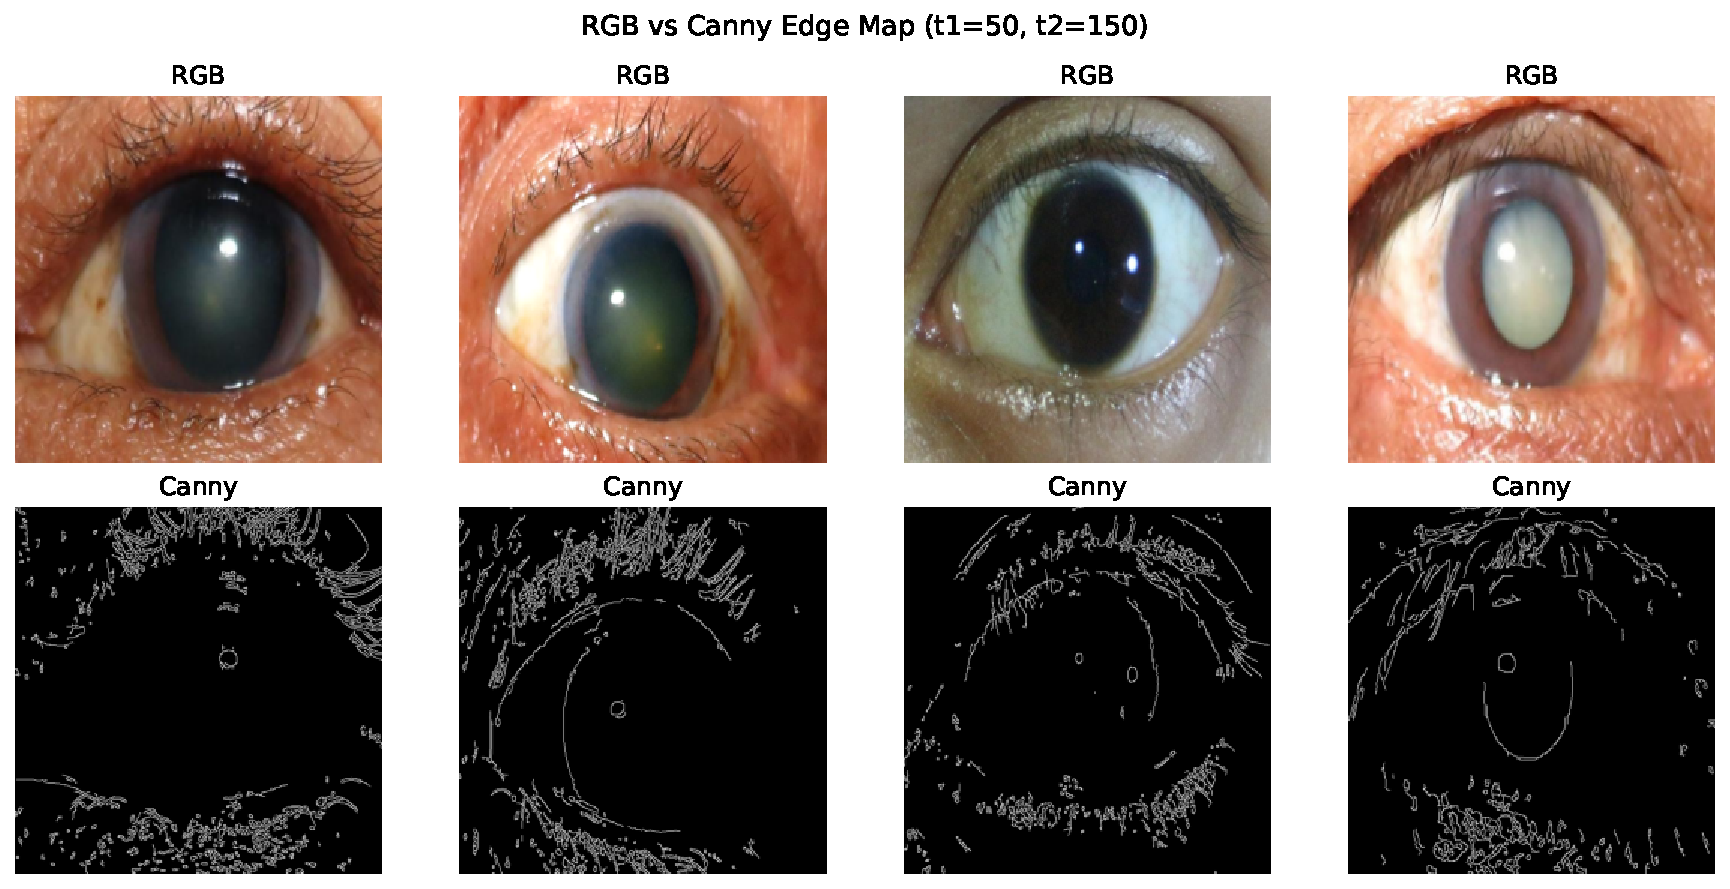
\includegraphics[width=0.92\textwidth]{../figures/canny_visualization.pdf}
\vspace{0.3em}

{\small \textbf{Fila superior:} imágenes RGB originales \quad \textbf{Fila inferior:} mapas de bordes Canny ($t_1{=}50$, $t_2{=}150$)}\\[0.2em]
{\small Los bordes del cristalino y la córnea son geométricamente explícitos incluso cuando el contraste de color es bajo.}
\end{frame}

% ── Slide 12: Encoders duales ─────────────────────────────────────────────────
\begin{frame}{Encoders Duales}
\begin{itemize}
    \item Dos encoders U-Net \textbf{independientes} — misma arquitectura ResNet-34, \textbf{sin pesos compartidos}
    \vspace{0.3em}
    \item Cada encoder produce mapas de features en \textbf{5 resoluciones}:
    \begin{itemize}
        \item Canales: 64 → 64 → 128 → 256 → 512
        \item Resolución espacial: 256 → 128 → 64 → 32 → 16
    \end{itemize}
    \vspace{0.3em}
    \item \textbf{Encoder A} procesa la imagen RGB
    \item \textbf{Encoder B} procesa el mapa de bordes
\end{itemize}
\vspace{0.3em}
\begin{block}{Clave}
Los pesos separados permiten que cada encoder aprenda representaciones especializadas para su modalidad.
\end{block}
\end{frame}

% ── Slide 12: Módulo de Cross-Attention ──────────────────────────────────────
\begin{frame}{Módulo de Cross-Attention}
\begin{columns}
\column{0.55\textwidth}
Reshape: $(B, C, H, W) \rightarrow (B,\, HW,\, C)$

\vspace{0.4em}
\begin{equation*}
\tilde{\mathbf{F}}_A = \text{LN}\!\left(\alpha \cdot \text{MHA}(\underbrace{Q{=}\mathbf{F}_A}_{\text{RGB}},\; \underbrace{K{=}V{=}\mathbf{F}_B}_{\text{bordes}}) + \mathbf{F}_A\right)
\end{equation*}

\vspace{0.3em}
\begin{itemize}
    \item \textbf{Q} viene del encoder RGB
    \item \textbf{K, V} vienen del encoder de bordes
    \item El encoder RGB \textbf{consulta} los features de bordes
    \item 8 cabezas de atención
\end{itemize}

\column{0.42\textwidth}
\begin{block}{¿Qué logra esto?}
Enriquece la representación fotométrica con información estructural geométrica antes del decodificador.
\end{block}
\end{columns}
\end{frame}

% ── Slide 13: Gate aprendible ─────────────────────────────────────────────────
\begin{frame}{Gate Escalar Aprendible}
\begin{columns}
\column{0.55\textwidth}
\begin{equation*}
\alpha = \sigma(\theta), \quad \theta_0 = -4 \Rightarrow \alpha_0 \approx 0.02
\end{equation*}
\vspace{0.3em}
\begin{itemize}
    \item Al inicio: modelo casi puramente RGB
    \item Durante el entrenamiento: $\alpha$ crece \textbf{solo si los bordes ayudan}
    \item Si el mapa Canny es ruidoso: el gate permanece cerrado
\end{itemize}

\column{0.42\textwidth}
\begin{alertblock}{¿Por qué es importante?}
Sin el gate, los features de bordes ruidosos degradarían el rendimiento. El gate protege al modelo.
\end{alertblock}
\vspace{0.3em}
\begin{block}{Diferencia con Early Fusion}
Early Fusion fuerza ambas modalidades desde la época 1. El gate es selectivo.
\end{block}
\end{columns}
\end{frame}

% ── Slide 14: Fusión multi-escala ─────────────────────────────────────────────
\begin{frame}{Fusión Multi-Escala}
\textbf{Dos instancias de cross-attention:}
\vspace{0.3em}
\begin{enumerate}
    \item \textbf{Cuello de botella} — 512 canales, resolución $16{\times}16$
    \item \textbf{Etapa 4} — 256 canales, resolución $32{\times}32$
\end{enumerate}
\vspace{0.5em}
\textbf{Skip connections del encoder de bordes:}
\begin{equation*}
\hat{\mathbf{F}}^{(s)} = \text{Conv}_{1\times1}\!\left(\left[\mathbf{F}_A^{(s)} \;\|\; \mathbf{F}_B^{(s)}\right]\right), \quad s \in \{1,2,3,4\}
\end{equation*}
\vspace{0.2em}
\begin{block}{Efecto combinado}
Los cues geométricos se propagan por \textbf{todo el camino de expansión}, no solo en el cuello de botella.
\end{block}
\end{frame}

% ── Slide 15: Entrenamiento ───────────────────────────────────────────────────
\begin{frame}{Configuración de Entrenamiento}
\begin{columns}
\column{0.48\textwidth}
\textbf{Función de pérdida}
\begin{equation*}
\mathcal{L} = \mathcal{L}_\text{BCE} + \mathcal{L}_\text{Dice}
\end{equation*}
Penaliza errores a nivel de píxel y de solapamiento

\vspace{0.4em}
\textbf{Optimizador:} AdamW\\
lr $= 10^{-4}$, weight decay $= 10^{-2}$

\vspace{0.4em}
\textbf{Schedule:} 100 épocas, batch 8

\column{0.48\textwidth}
\textbf{Augmentación (solo entrenamiento)}
\begin{itemize}
    \item Flip horizontal ($p = 0.5$)
    \item Rotación $\pm 15°$
    \item Jitter de brillo/contraste $[0.8, 1.2]$
    \item Mapa de bordes \textbf{recalculado} tras transforms geométricas
\end{itemize}

\vspace{0.3em}
\textbf{Hardware:} NVIDIA A100 40GB (Colab)\\
\textbf{Semilla:} 42 (todas las corridas)
\end{columns}
\end{frame}

% ══════════════════════════════════════════════════════════════════════════════
%  DANILO — Slides 16–23  (~6 min)
% ══════════════════════════════════════════════════════════════════════════════

% ── Slide 16: Dataset ─────────────────────────────────────────────────────────
\begin{frame}{Dataset: Cataract-Seg}
\begin{columns}
\column{0.5\textwidth}
\begin{itemize}
    \item \textbf{Fuente:} Roboflow Universe (Muhammad Risma, 2023)
    \item Imágenes de segmento anterior con máscaras de píxeles
    \item Estructuras: córnea, pupila, cristalino
\end{itemize}
\vspace{0.4em}
\textbf{Partición estratificada 70/15/15:}
\begin{center}
\begin{tabular}{lc}
\hline
Split & Imágenes \\
\hline
Entrenamiento & 210 \\
Validación    & 45  \\
\textbf{Test} & \textbf{45}  \\
\hline
\end{tabular}
\end{center}

\column{0.46\textwidth}
\textbf{4 modelos comparados:}
\vspace{0.3em}
\begin{tabular}{ll}
\hline
Modelo & Entrada \\
\hline
U-Net (RGB) & Solo RGB \\
U-Net (Bordes) & Solo bordes \\
U-Net (Fusión T.) & RGB+bordes concat. \\
\textbf{Propuesto} & Encoder dual + attn \\
\hline
\end{tabular}
\vspace{0.3em}

{\small Mismo backbone, optimizador y schedule para comparación justa.}
\end{columns}
\end{frame}

% ── Slide 17: Métricas ────────────────────────────────────────────────────────
\begin{frame}{Métricas de Evaluación}
\begin{itemize}
    \item \textbf{IoU (Intersection over Union)} — métrica primaria
    \begin{equation*}
        \text{IoU} = \frac{|\hat{M} \cap M|}{|\hat{M} \cup M|}
    \end{equation*}
    Penaliza tanto falsos positivos como falsos negativos
    \vspace{0.4em}
    \item \textbf{Dice / F1} — métrica secundaria
    \begin{equation*}
        \text{Dice} = \frac{2|\hat{M} \cap M|}{|\hat{M}| + |M|}
    \end{equation*}
    Equivalente a F1 en segmentación binaria
\end{itemize}
\end{frame}

% ── Slide 18: Resultados cuantitativos ───────────────────────────────────────
\begin{frame}{Resultados Cuantitativos}
\centering
\begin{tabular}{lcc}
\hline
\textbf{Modelo} & \textbf{IoU} & \textbf{Dice/F1} \\
\hline
U-Net (RGB)            & 0.9529 & 0.9759 \\
U-Net (Bordes)         & 0.8817 & 0.9371 \\
U-Net (Fusión T.)      & \textbf{0.9532} & \textbf{0.9761} \\
\textbf{Propuesto}     & 0.9530 & 0.9759 \\
\hline
\end{tabular}
\vspace{0.5em}
\begin{itemize}
    \item Los bordes solos confirman que Canny no es suficiente de forma independiente (IoU 0.88)
    \item Los 3 modelos basados en RGB están dentro de \textbf{0.0003 IoU} — ruido estadístico a $n=45$
    \item El modelo propuesto \textbf{empata en primer lugar} con un mecanismo más principiado
\end{itemize}
\end{frame}

% ── Slide 19: Gráfico IoU ─────────────────────────────────────────────────────
\begin{frame}{Comparación de IoU en Test}
\centering
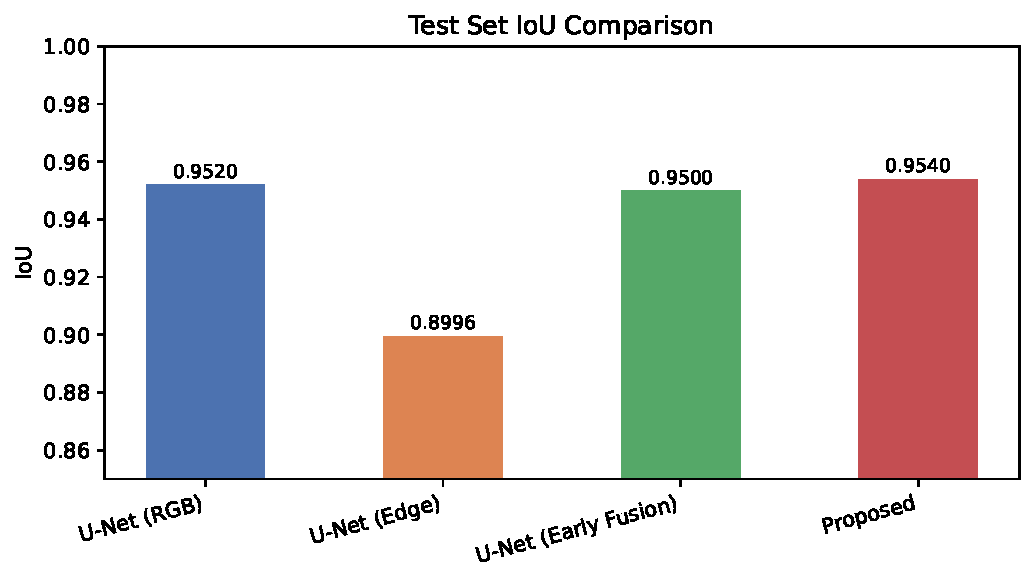
\includegraphics[width=0.75\textwidth]{../paper/figures/iou_comparison.pdf}
\vspace{0.3em}

{\small Eje Y desde 0.85 para ampliar diferencias. La brecha principal es entre bordes solos y los modelos RGB.}
\end{frame}

% ── Slide 20: Curvas de pérdida ──────────────────────────────────────────────
\begin{frame}{Curvas de Pérdida}
\centering
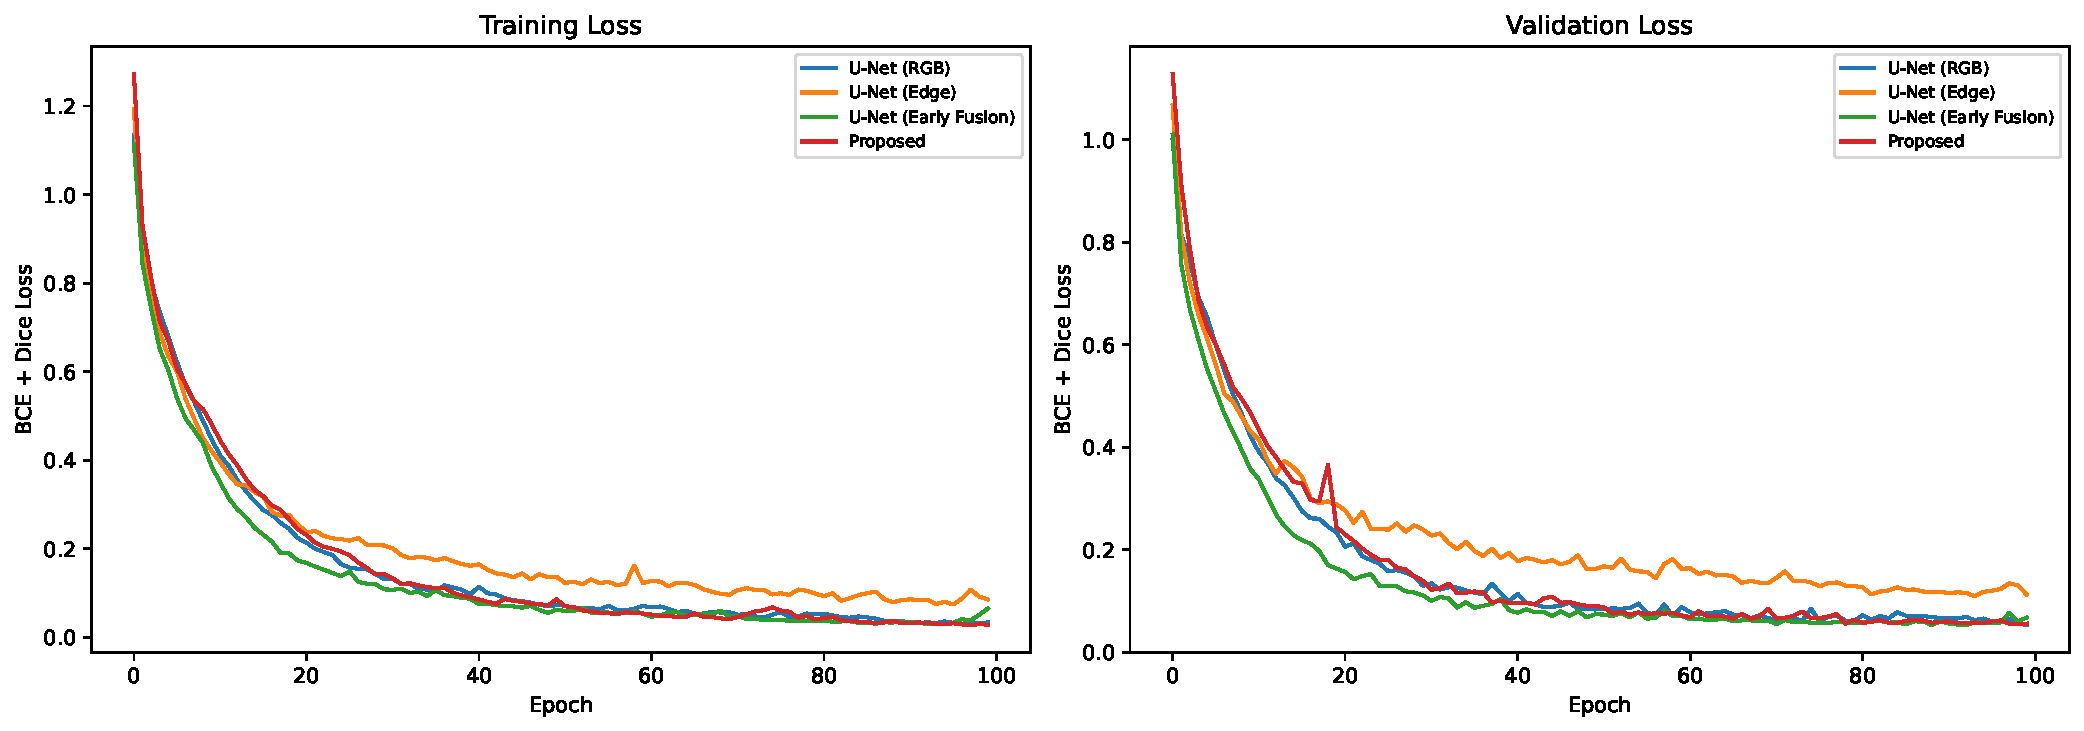
\includegraphics[width=0.85\textwidth]{../paper/figures/loss_curves.pdf}
\vspace{0.3em}

{\small Pérdida BCE+Dice de entrenamiento (izq.) y validación (der.) — 100 épocas. Todos los modelos convergen sin divergencia.}
\end{frame}

% ── Slide 21: Curvas de IoU de validación ────────────────────────────────────
\begin{frame}{IoU de Validación por Época}
\centering
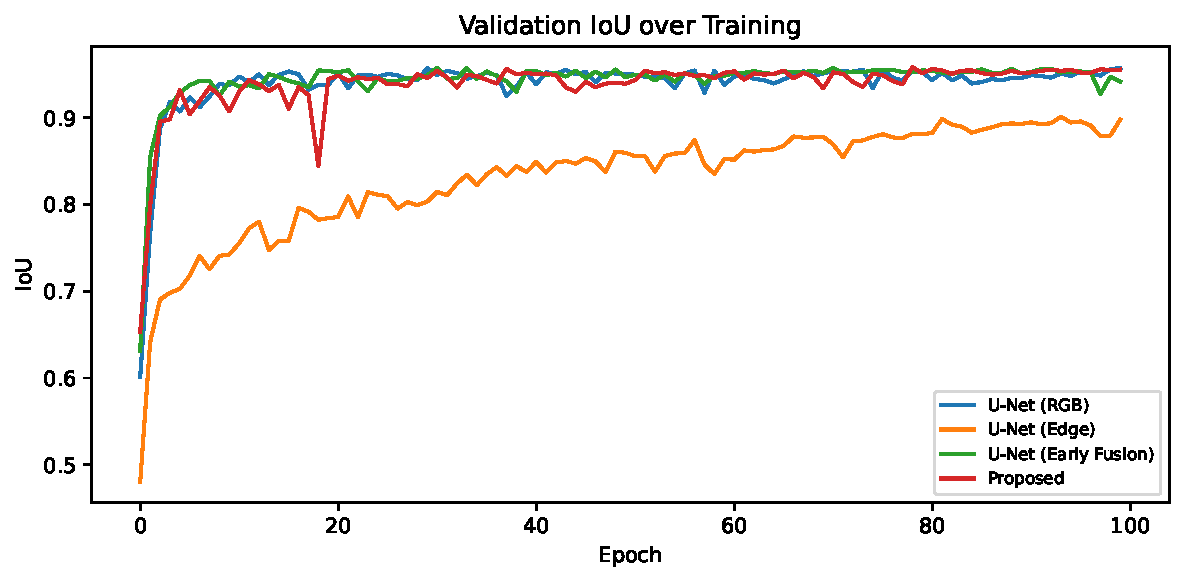
\includegraphics[width=0.82\textwidth]{../paper/figures/val_iou_curves.pdf}
\vspace{0.3em}

{\small El modelo propuesto y Fusión Temprana siguen trayectorias paralelas. Bordes solos: meseta más baja.}
\end{frame}

% ── Slide 22: Predicciones cualitativas ──────────────────────────────────────
\begin{frame}{Predicciones Cualitativas}
\centering
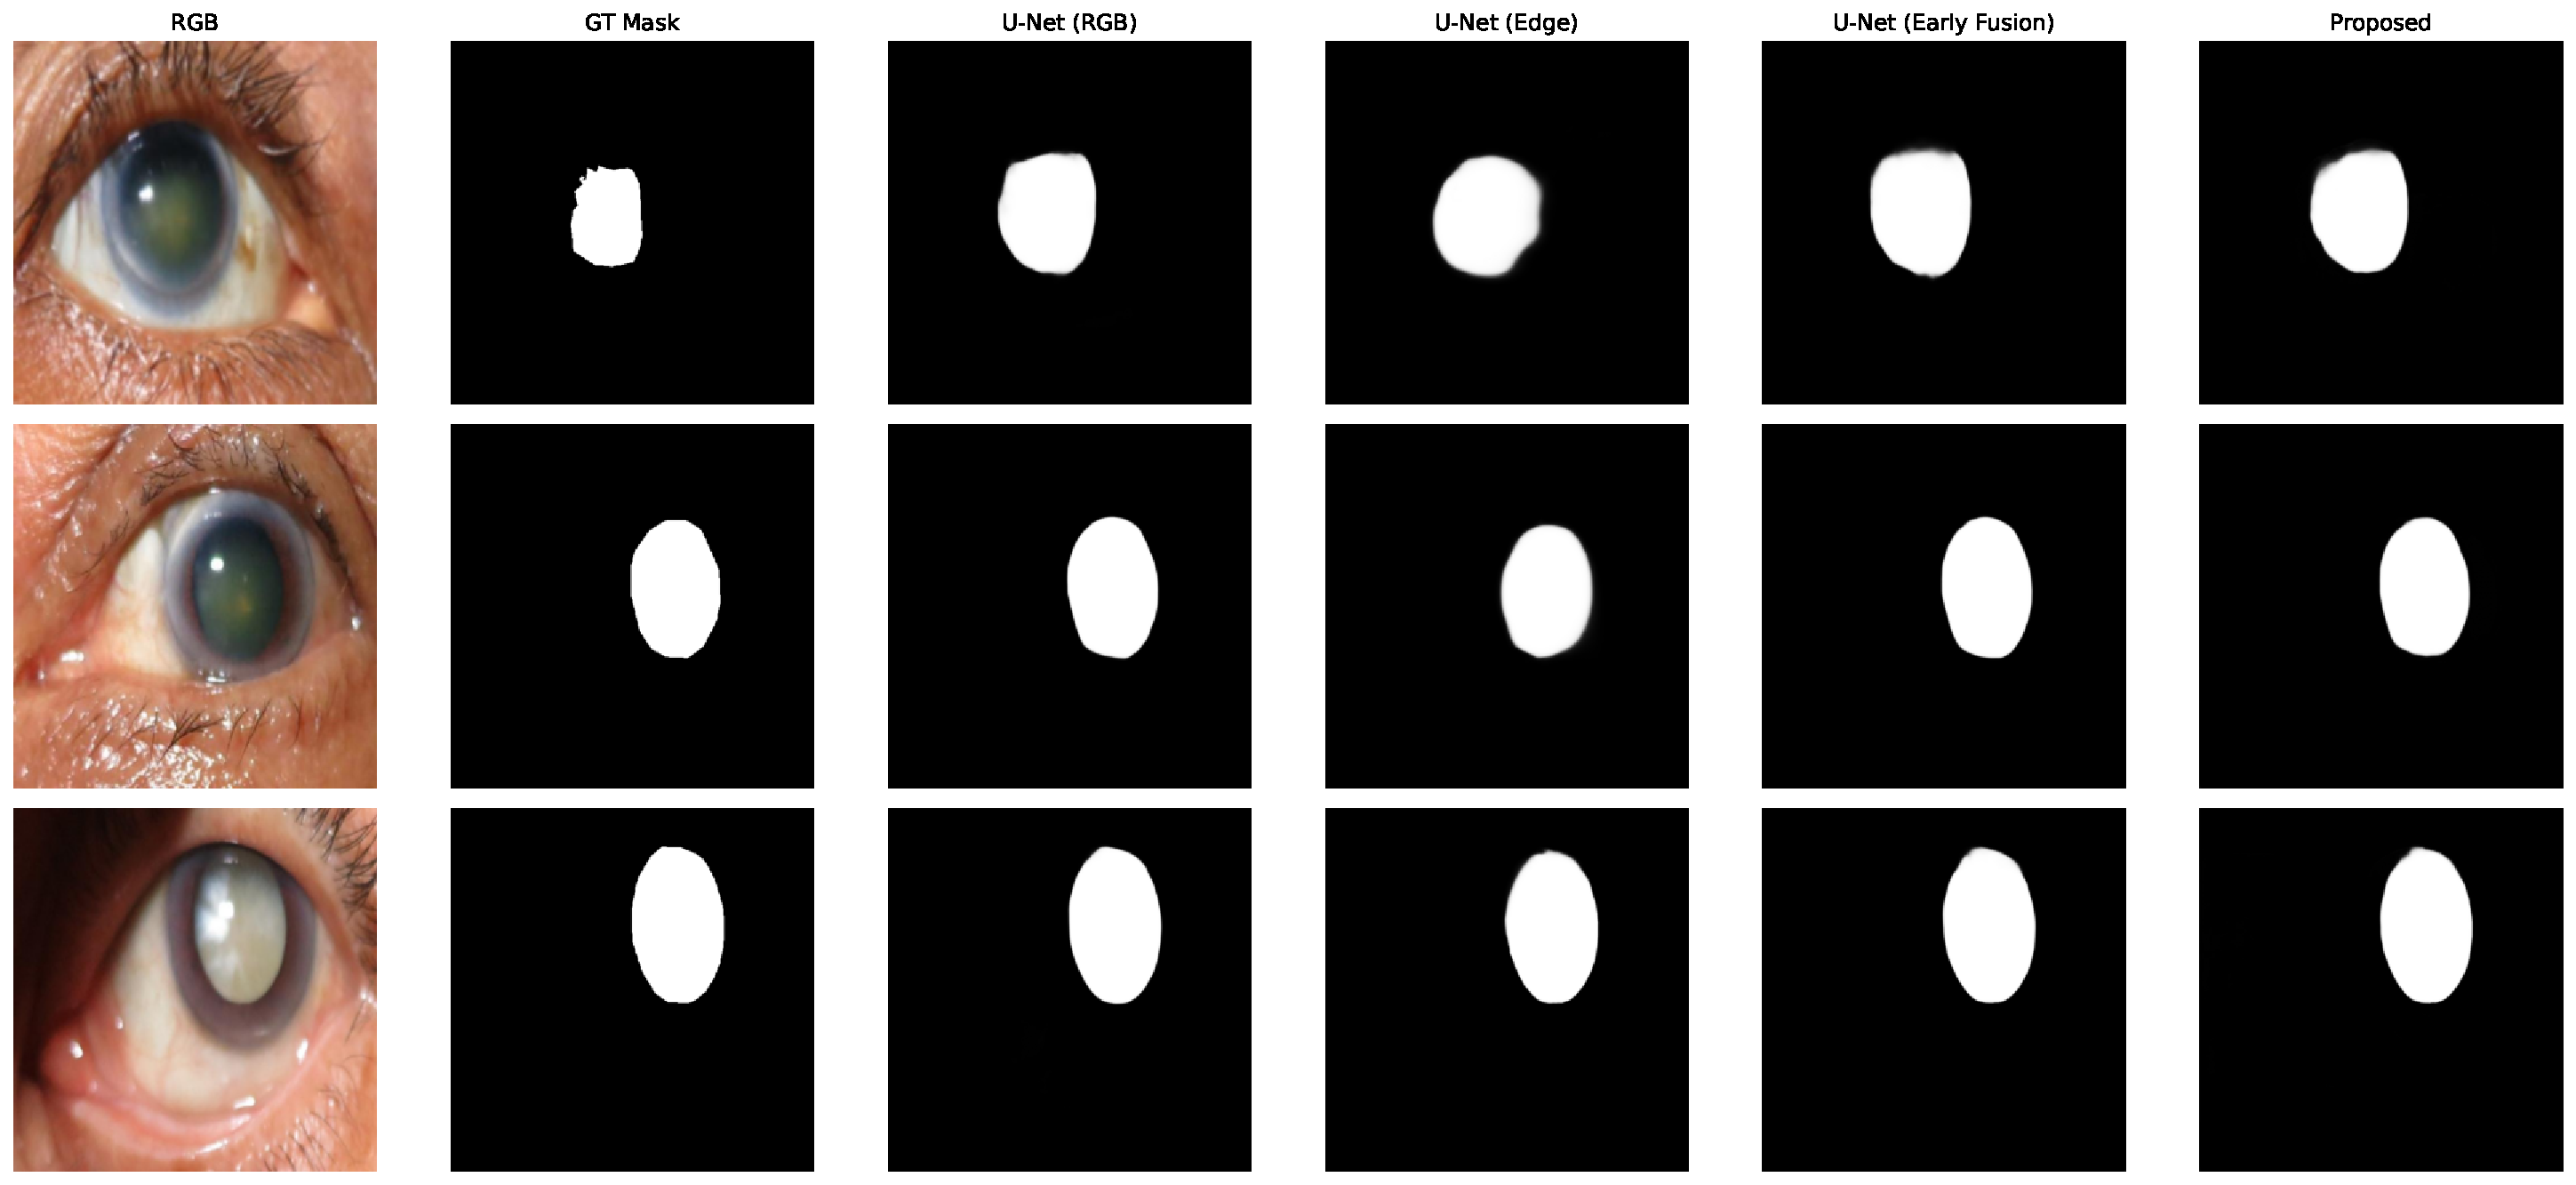
\includegraphics[width=0.95\textwidth]{../paper/figures/qualitative_predictions.pdf}

{\small \textbf{Columnas:} RGB — GT — U-Net RGB — U-Net Bordes — Fusión T. — \textbf{Propuesto}}\\[0.2em]
{\small Bordes solos: contornos más gruesos y ruidosos. Los modelos RGB: máscaras visualmente similares.}
\end{frame}

% ── Slide 23: Conclusión — título ────────────────────────────────────────────
\begin{frame}{Conclusión}
\centering
\vspace{2em}
{\Large Tres contribuciones arquitectónicas.\\[0.5em] Un resultado competitivo.}
\end{frame}

% ── Slide 24: Lo que hicimos ──────────────────────────────────────────────────
\begin{frame}{Conclusión: Lo que Hicimos}
\begin{itemize}
    \item Encoder dual U-Net: RGB + mapa de bordes Canny
    \vspace{0.4em}
    \item Cross-attention con gate aprendible en cuello de botella + etapa 4
    \vspace{0.4em}
    \item Skip connections del encoder de bordes en todos los niveles del decodificador
\end{itemize}
\vspace{0.5em}
\begin{alertblock}{Limitaciones}
\begin{itemize}
    \item Test set de 45 imágenes — diferencias dentro del ruido estadístico
    \item Umbrales Canny fijos
    \item Sin tabla de ablación
\end{itemize}
\end{alertblock}
\end{frame}

% ── Slide 25: Lo que logramos ─────────────────────────────────────────────────
\begin{frame}{Conclusión: Lo que Logramos}
\begin{itemize}
    \item \textbf{0.9530 IoU} — empatado con el mejor baseline
    \vspace{0.4em}
    \item Fusión robusta al ruido gracias al gate aprendible
    \vspace{0.4em}
    \item Reproducible: A100, semilla 42, código en GitHub
\end{itemize}
\end{frame}

% ── Slide 23: Gracias ─────────────────────────────────────────────────────────
\begin{frame}{}
\centering
\vspace{2em}
{\LARGE \textbf{¡Gracias!}}\\[1.5em]
{\large ¿Preguntas?}\\[2em]
\texttt{github.com/DaniloDuque/multimodal-cataract-seg}
\end{frame}

\end{document}
